Замеры проводились 10 раз, каждый раз моделировался процесс обработки 300 запросов. Проводился подсчёт обслуженных и отказанных заявок, а также времени моделирования, и по результатам вычислялась вероятность, с которой клиенту могут отказать в обработке его заявки. Результаты приведены на рисунке \ref{fig3:image}.

\begin{figure}[h]
	\begin{center}
		{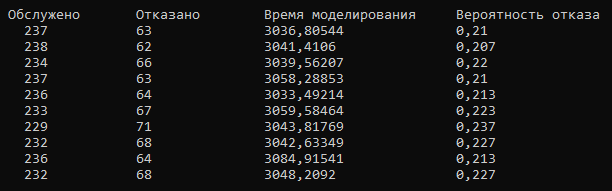
\includegraphics[scale = 0.9]{img/results.png}}
		\caption{Результаты замеров}
		\label{fig3:image}
	\end{center}
\end{figure}